\chapter{Design}\label{ch:design}

This section discusses the design of the system. The first part explains query
spawning and execution, the second part describes how data stream can be shared
between queries.

\section{Overall Architecture}

Our system consists of multiple components which are briefly described in this
paragraph. A dataflow program submitted to run as part of the system is
called a \emph{query}. Following Timely's terminology, the execution of a query
is done by a group of \emph{worker} threads. Each worker manages the scheduling and
notification of the nodes that are part instance of the dataflow graph. 

A query is executed by one or more \emph{executors}. Each executor selected to
execute a query will fetch and invoke the query binary, ultimately spawning the
worker threads. 

All these components are managed by a process called the \emph{coordinator},
which stores the system state in the \emph{catalog}.

\section{Coordinator}

The coordinator is the central process managing all the components
of the system. In order to receive commands and report their internal state,
every executor and query process maintains a network connection to the coordinator.

Bookkeeping of the system is done by the coordinator in the catalog. The
catalog is a datastructure which contains all information about the available
executors, the running queries and their workers. 

\begin{figure}[htb]
  \centering
    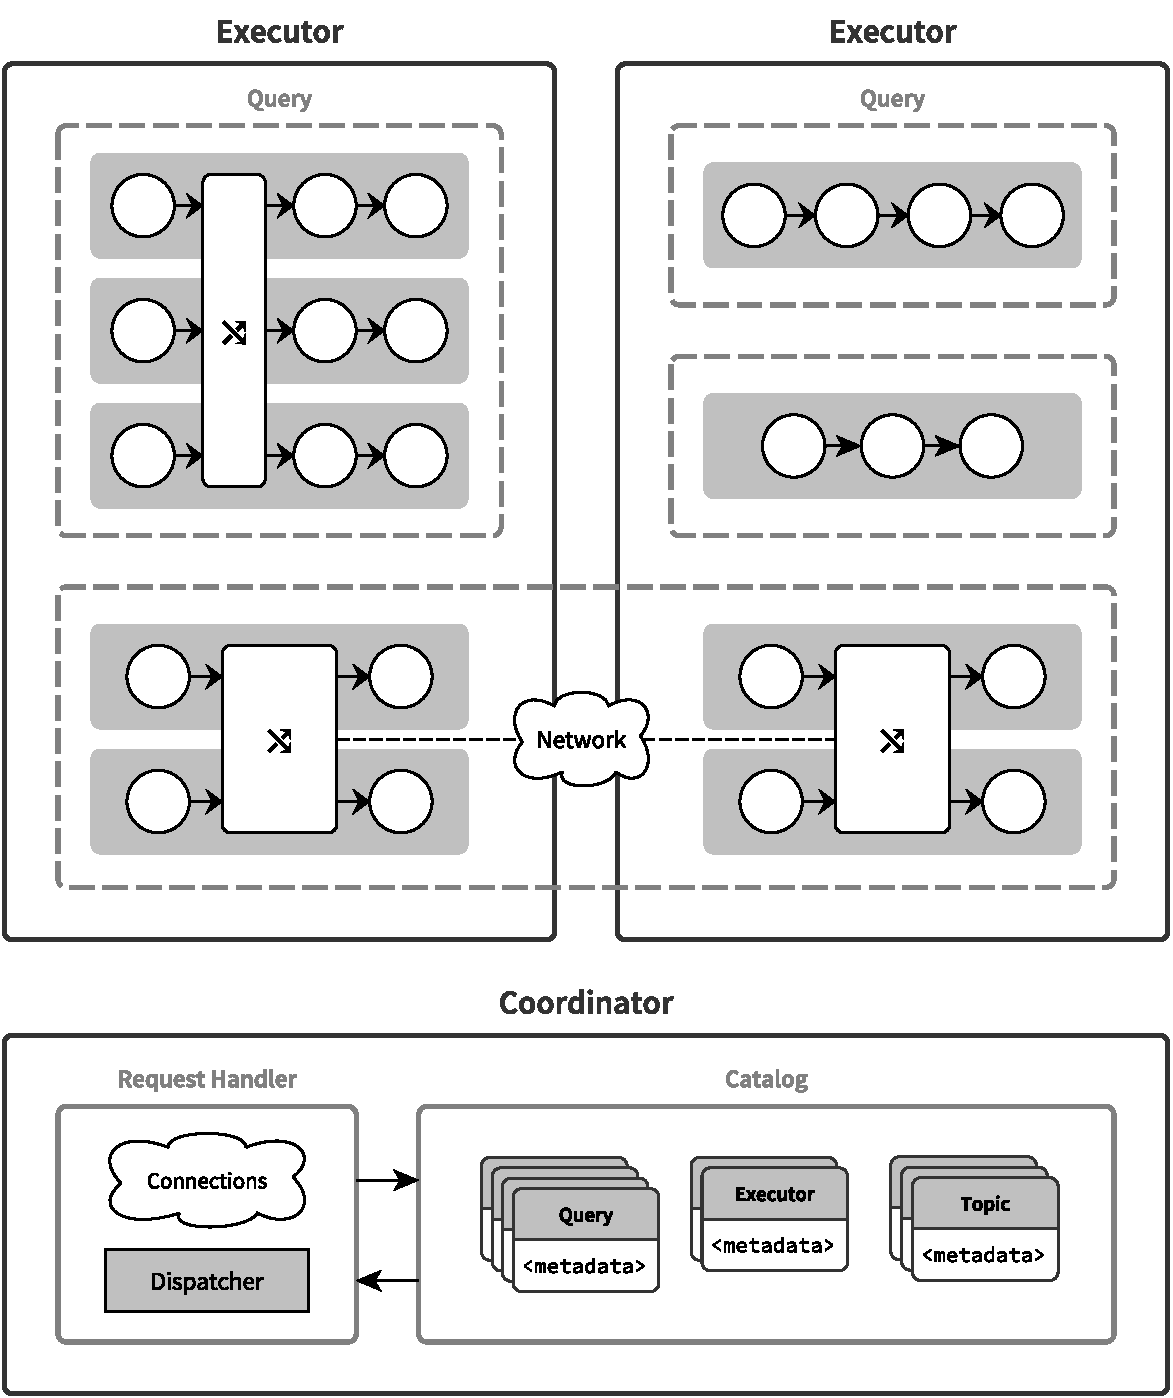
\includegraphics[width=1\textwidth]{figures/components}
  \caption[System architecture.]{ Queries (dashed boxes) consist of one or
  more worker threads (rounded grey boxes) driving the dataflow computation.
  A query might span over multiple executors, make use of the network for message exchanges
  between the workers of a query.\\
  The coordinator maintains a connection to every  executor and every query process.
  The state of the whole system is stored in the catalog.}
  \label{fig:components}
\end{figure}

\clearpage

\section{Queries}

A query is a Timely program managed and executed by our system. Like
standalone Timely Dataflow programs, queries are written in Rust by using the
Timely library: The dataflow graph is constructed by connecting
Timely's operators (vertices) to stream objects (edges).

In order for a Timely Dataflow program to become a runnable query on the system,
it needs to register its computational logic with with our system library instead of
using Timely Dataflow's initialization function. This
\lstinline{timely_query::execute} function not only performs the initialization
for the query, it also provides additional functionality to interact with the
coordinator. Other than this, there are no no restrictions on the query program,
it might execute arbitrary code.

\begin{lstlisting}[caption={[Example query.]Example query which creates a stream of integers,
filters out all odd numbers and then prints the rest.}]
extern crate timely;
extern crate timely_query;

use timely::dataflow::Scope;
use timely::dataflow::operators::{Filter, Inspect, ToStream};

fn main() {
    timely_query::execute(|root, catalog| {
        root.scoped::<u32, _, _>(|scope| {
            (0..100).to_stream(scope)
                .filter(|x| x % 2 == 0)
                .inspect(|x| println!("hello {:?}", x));
        });
    }).unwrap();
}
\end{lstlisting}

\subsection{Submission}

A query is submitted to the coordinator as a binary executable. A submission
consists of an URL and format of the query binary, as well as the runtime
configuration for the workers. The runtime configuration specifies the amount
and distribution of the worker threads which will drive the query.

Optionally, a human-readable description of the query,
as well as the command-line arguments to be passed to the executable can be
provided. (TODO: this is currently not implemented)

When handling a new query submission request, the coordinator will assign a
unique identifier to the incoming query, and then select a
matching number of executors for the query to be spawned on. The selection
of executors is based on the runtime configuration provided by the submission
request.

The coordinator plays a important role when spawning new queries. After
issuing query spawn requests to the executors, it waits for all query processes
to register themselves at the coordinator before they begin their computation.
Only then the query is considered active and the submission request
is reported to be completed.


\section{Executors}

Executors are a processes responsible for query spawning and supervision. Typically,
every machine supposed to host query processes will require an executor
instance. Executors register themselves at the coordinator, telling it the type
of binary they are able to execute. 

Executors, and thus machines, can easily be added to the system and can be used
to host new incoming queries. Due to how Timely implements its worker allocation,
it is not possible to extend already running queries to newly added executors.
Depending on the implementation of the executor, it might also be able to
deregister itself without terminating the query process it spawned.

If there is a new query to be executed on an executor, the coordinator will notify
it. The notified executor will then fetch the query binary from the specified URL
and typically spawn it as a new process.

When spawning a new query process, the executor will also supply the newly created
process with the information the process needs in order to participate as a query:
The address of the coordinator, the address of any peer processes belonging to the 
same query, the number of worker threads to spawn and the query's own identifier.

\section{}

Pubsub
